The standard model of particle physics (SM) describes various phenomena of particle physics.
The discovery of the Higgs boson ($H$) by the ATLAS and CMS collaboration at CERN completes the missing part of the SM prediction~\cite{Aad:2012tfa, Chatrchyan:2012xdj}.
However, there are several open challenges that cannot be explained by the SM, such as hierarchy problem~\cite{Weinberg:1975gm, Gildener:1976ai, Susskind:1978ms} and the dark matter candidate.
In order to answer those questions, a new theory extending the SM is necessary.
Supersymmetry (SUSY)~\cite{Wess:1973kz, Wess:201649, Golfand:1971iw, Martin:1997ns} is the most promising extensions of the SM.
SUSY, which is a spacetime symmetry, introduces the superpartners of SM particles (sparticles) with spin differing by one-half unit with respect to the SM partners.
The sparticles provide a potential solution to the hierarchy problem.
If $R$-parity is conserved~\cite{Fayet:1976et, Fayet:1977yc, Farrar:1978xj}, the sparticles are produced in pairs and the lightest SUSY particle (LSP) is stable providing the candidate for dark matter.

The charginos $\tilde{\chi}^{\pm}_{1,2}$ and neutralinos $\tilde{\chi}^{0}_{1,2,3,4}$ are the mass eigenstates in the order of increasing masses and collectively refferred to as electroweakinos.
They are the mixture of the bino $\tilde{B}$, winos $\tilde{W}$, and higgsinos $\tilde{H}_{u,d}$ which are the superpartners of the $U(1)$, $SU(2)$ gauge bosons, and the Higgs bosons, respectively.
The charginos and neutralinos can decay into leptons and LSPs via $W, Z, H$ or sleptons $\tilde{\ell}$.
In many SUSY models, the lightest neutralino $\tilde{\chi}^{0}_{1}$ is the LSP.
The LSP couldn't be detected and results in significant missing transverse energy \MET.

The compressed scenarios refer to the small mass differences between heavier SUSY particles and the LSP.
For example, the mass differences between the heavier electroweakino states $\tilde{\chi}^{0}_{2}$, $\tilde{\chi}^{\pm}_{1}$ and the wino- or higgsino-dominated LSP $\tilde{\chi}^{0}_{1}$ range from a few {\MeV} to tens of {\GeV} depending on the composition of the mixture.
The $\tilde{B}, \tilde{W}$, and $\tilde{H}$ composition of the $\tilde{\chi}^{0}_{1}$ have an influence on the degree of compression.
Figure~\ref{fig:intro_LSP_composition} shows the composition of the lightest neutralino in a MSSM scan of the electroweakino sector~\cite{Aaboud:2016wna}.
Based on naturalness arguments~\cite{Barbieri:1987fn, deCarlos:1993rbr}, the Higgsino mass parameter $\mu$, the bino and wino mass parameters $M_{1}$ and $M_{2}$ satisfy $|\mu| \ll |M_{1}|, |M_{2}|$ leading to the three electroweakinos $\tilde{\chi}^{0}_{1}$, $\tilde{\chi}^{\pm}_{1}$, and $\tilde{\chi}^{0}_{2}$ being dominated by the Higgsino.

\begin{figure}[htbp]
\begin{center}
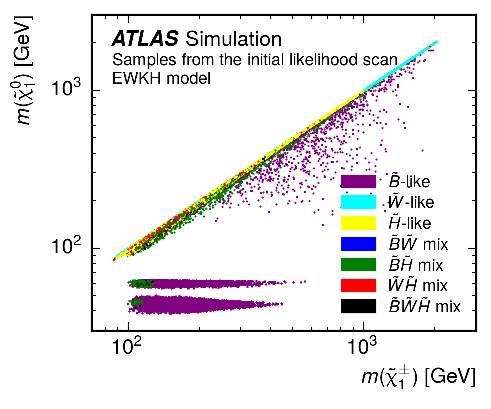
\includegraphics[scale=1.0]{LSP_composition.pdf}
\caption{The scatter plot in the $m(\tilde{\chi}^{0}_{1}$ vs $m(\tilde{\chi}^{\pm}_{1})$ plane.
The color encode the $\tilde{\chi}^{0}_{1}$ composition.
The Higgsino-dominated LSPs are colored in yellow and along the $\tilde{\chi}^{0}_{1}$-$\tilde{\chi}^{\pm}_{1}$ diagonal.
The figure is taken from~\cite{Aaboud:2016wna}.}
\label{fig:intro_LSP_composition}
\end{center}
\end{figure}